The Provisioning XEP is a protocol that focuses on the security aspect of IoT. Provisioning allows the delegation of user privileges and access rights from a provisioning server to the necessary nodes in a network to the users attempting to access them. The main goal of Provisioning is to be implementable for small devices with limited memory and UI options. This relates to IoT because many devices in the network will indeed have limited memory and UI options. \\
The specification for the Provisioning XEP, provides a means of establishing a `trust relationship' between a provisioning server and a sensor with only a single button, LED, and several methods implemented to interact with a provisioning server. The sensor is given a connection to an XMPP server and an id, and the server is notified to create a `presence subscription request' to the sensor. Receiving the first presence subscription request, the sensor flashes its LED and the user installing the sensor presses the button, therefore accepting the request. The sensor now knows of the existence of the provisioning server. The sensor can then query the server to see if it has provisioning implemented. Once it realizes that it does, and that it is communicating with the server, it requests a token to identify itself with for the server. This token is the device's key to accessing methods of other nodes in the network. The sequence diagram, Figure 2.1 below, illustrates the successful case of delegating trust to the provisioning server. \\
\begin{figure*}
\centering
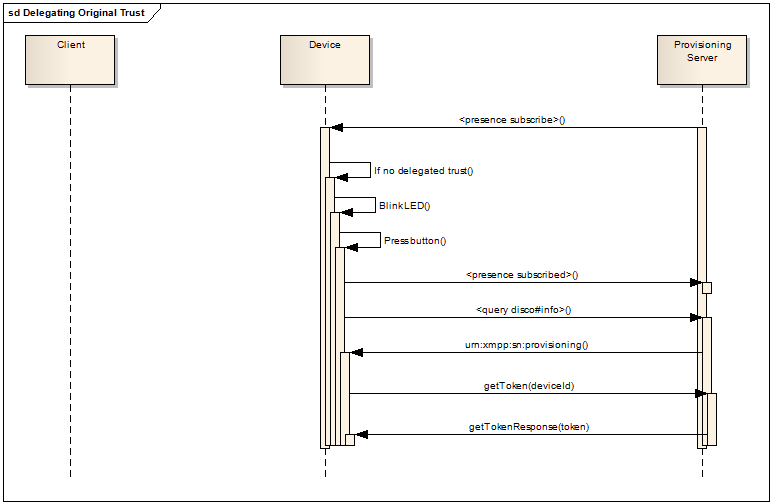
\includegraphics[scale=.5]{images/delegatingTrustSimpleNode}
\caption{Provisioning Server Presence Subscription Request}
\end{figure*}
A token is not solely for the use of a device. Provisioning servers give tokens to services as well, who will use them for set and read commands. Once a provisioning server is installed and running in a network, all devices supporting Control/Sensor Data can be set to require a token if given a command. That way when a service executes a set or read command on a device, its token and command will be passed onto the provisioning server. The server will denote if the given service (and/or human user behind that service) has privileges to run the given command. This is also known as the hasPrivilege query.\\
Since the token is a powerful identification tool, the Provisioning Server has a means of challenging the token to ensure that the device is not spoofing its identity whenever it makes requests using the token. This is possible because the initial call to getToken has a single parameter that is the public part of a Base-64 Public X.509 Certificate. To challenge the device, the provisioning server encrypts a challenge using the public part of the certificate that it received from the original call of getToken and sends the challenge to the device. The device then decrypts the challenge using the private part of the certificate and returns it to the server. \\
Provisioning also has friendships, or the right to send commands to a given device. Upon receiving a presence subscription from a client, a device will ask the provisioning server if the client is its friend. If the server responds with yes, then the device will allow the client to send it commands. If the server responds with no, they have the option to allow the device to add its own friends through a concept called secondary trust.\\
If a device is granted secondary trust, it essentially may converse with anyone that it wishes to. If the device A makes can send commands to other another device B, then essentially any friend that A adds is inherently a friend of B. Due to the unavoidable relationship of the new friend to the B device, XMPP authors warn the reader that secondary trust should be handled with caution.\\
